\documentclass[spanish]{article}
\usepackage{graphicx}
\usepackage{ragged2e}
\usepackage{geometry}
\usepackage{float}
\usepackage{hyperref}
\usepackage[table,xcdraw]{xcolor}
\usepackage[ruled,vlined]{algorithm2e}
\title {Práctica 4: Divide y Venceŕas}
\graphicspath{{../img/}}
\addtolength{\textheight}{1.5in} 
\begin{document}
	\centerline{
\includegraphics[width=450px,height=100px]{header}}
	\centerline{Analisis de algoritmos, Sem: 2021-1, 3CV1,Práctica  3, 11/11/2020}
	\centering{\huge{Práctica 4: Divide y Venceŕas}}
	\centerline{\newline{\textbf{Payán Téllez René}}}
	\newline{\textit{rpayant1500@alumno.ipn.mx}}
	\bigskip
	\justify
	\textbf{Resumen:}	
	En esta practica se analizaran 2 algoritmos que utilizan la tecnica de divide y venceras para resolver un problema, uno de ellos el quick sort y otro el sub arreglo maximo.\\
	\textbf{Palabras clave:}
	QuickSort,SubArreglo maximo,divide y venceras,C/C++
	\section{Introduccion}
	
	\section{Conceptos Basicos}
	\subsection{Algoritmo}
	La palabra algoritmo proviene del sobrenombre de un matemático árabe del siglo IX, Al-Khwarizmi, que fue reconocido por enunciar paso a paso las reglas para las operaciones matemáticas básicas con decimales (suma, resta, multiplicación y división).	
	Vemos definición de algoritmo como un grupo de órdenes consecutivas que presentan una solución a un problema o tarea. Algunos ejemplos de algoritmos los podemos encontrar en las matemáticas (como el algoritmo para resolver una multiplicación) y en los manuales de usuario de un aparato (como una lavadora o una impresora).	
	Sin embargo, hoy en día se relaciona la palabra algoritmo con el mundo de la informática, más concretamente en la programación; los conocidos como algoritmos informáticos.[1]
	\subsection{Divide y venceras}	
	El  término  Divide  y  Vencerás  en  su  acepción  más  amplia  es  algo  más  que  una  técnica  de  diseño  de  algoritmos.  De  hecho,  suele  ser  considerada  una  filosofía  general  para  resolver  problemas  y  de  aquí  que  su  nombre  no  sólo  forme  parte  del  vocabulario informático, sino que también se utiliza en muchos otros ámbitos.      En nuestro contexto, Divide y Vencerás es una técnica de diseño de algoritmos que  consiste  en  resolver  un  problema  a  partir  de  la  solución  de  subproblemas  del  mismo tipo, pero de menor tamaño. Si los subproblemas son todavía relativamente grandes   se   aplicará   de   nuevo   esta   técnica   hasta   alcanzar   subproblemas   lo   suficientemente  pequeños  para  ser  solucionados  directamente.  Ello  naturalmente  sugiere el uso de la recursión en las implementaciones de estos algoritmos.       La  resolución  de  un  problema  mediante  esta  técnica  consta  fundamentalmente  de los siguientes pasos: 1.   En   primer   lugar   ha   de   plantearse   el   problema   de   forma   que   pueda   ser   descompuesto  en  k  subproblemas  del  mismo  tipo,  pero  de  menor  tamaño.  Es  decir, si el tamaño de la entrada es n, hemos de conseguir dividir el problema en k  subproblemas  (donde  1  ≤k≤n),  cada  uno  con  una  entrada  de  tamaño  nk  y  donde 0 ≤nk < n. A esta tarea se le conoce como división. 2.    En    segundo    lugar    han    de    resolverse    independientemente    todos    los    subproblemas,  bien  directamente  si  son  elementales  o  bien  de  forma  recursiva.  El hecho de que el tamaño de los subproblemas sea estrictamente menor que el tamaño  original  del  problema  nos  garantiza  la  convergencia  hacia  los  casos  elementales, también denominados casos base. 3.  Por  último,  combinar las soluciones obtenidas en el paso anterior para construir la solución del problema original.[1]	
	\subsection*{QuickSort}	
	\begin{algorithm}[H]
		\KwData{Entrada: N}
		\KwResult{Retorna el N-esimo termino de la serie de fibonacci}
		a=0\;
		b=0\;
		c=0\;
		\For{$i\gets1$ \KwTo $N$}{
			c = a\;
			a = b\;
			b += c\;
		}
		return a\;
		\caption{Solucion iterativa}
	\end{algorithm}
	\subsection*{Problema del maximo subarreglo}
	\begin{algorithm}[H]
		\KwData{Entrada: N}
		\KwResult{Retorna el N-esimo termino de la serie de fibonacci}
		\If{$N$ = 0}{
			return 0\;		
		}
		\ElseIf{$N$ = 1}{
			return 1\;
		}
		\Else{
			return 	solucionRecursiva($N$-1)+solucionRecursiva($N$-2);
		}
		\caption{Solucion recursiva}
	\end{algorithm}	
	\subsection*{Algoritmo de Karatsuba}	
	\section{Experimentacion y Resultados}
	\subsection{Implementar la sucecion de Fibonacci mediante un algoritmo recursivo y mediante unalgoritmo iterativo.}
	Se ejecuto el programa para encontrar los primeros 40 terminos de la sucesion de fibonacci con ambos algoritmos.			
	\begin{figure}[h!]
		\centering
		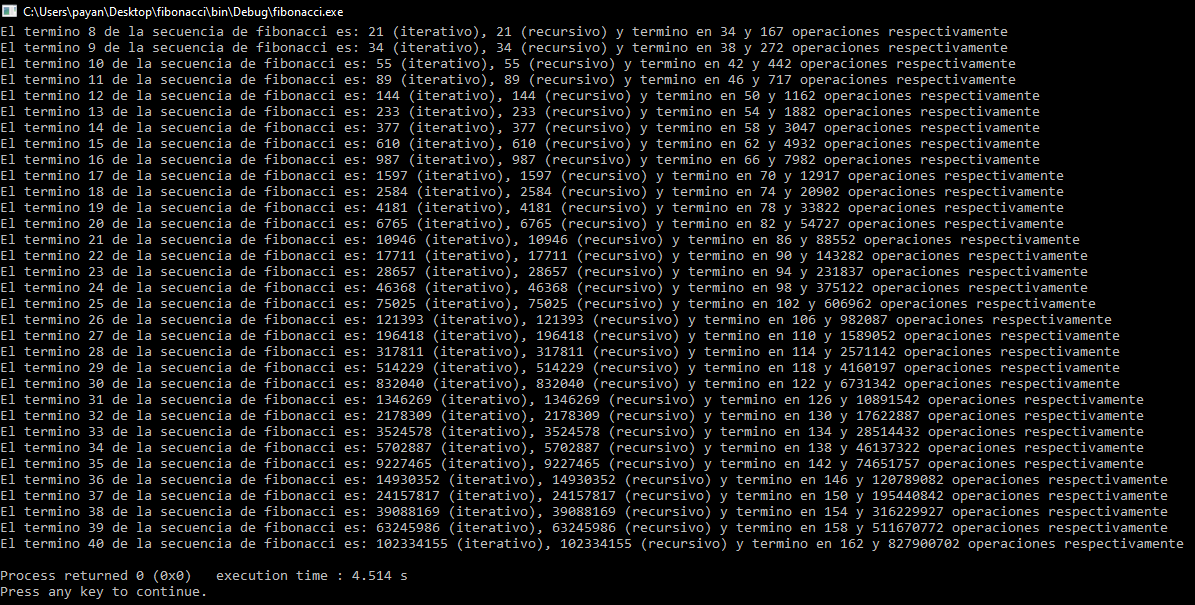
\includegraphics[width=400px,height=200px]{ejecucionPrimeraParte}
		\caption{Ejecucion del programa con ambos algoritmos, imprime $N$ y el resultado de ambas implementaciones}
	\end{figure}
	\begin{figure}[H]
		\centering
		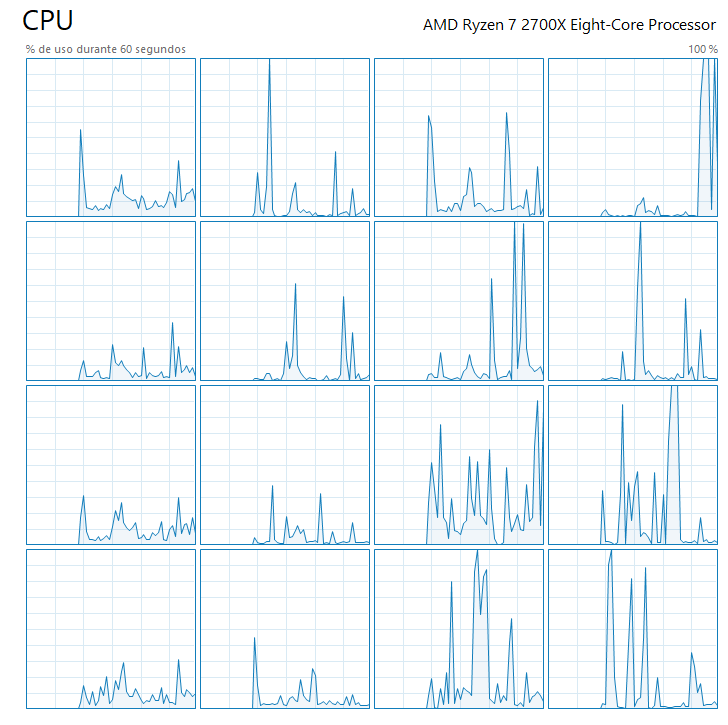
\includegraphics[width=400px,height=200px]{cpu}
		\caption{Como adicional, conforme aumentaba el valor del "limite", se incrementaba el tiempo que tardaba en terminar y el uso de CPU}
	\end{figure}
	\begin{figure}[H]
		\centering
		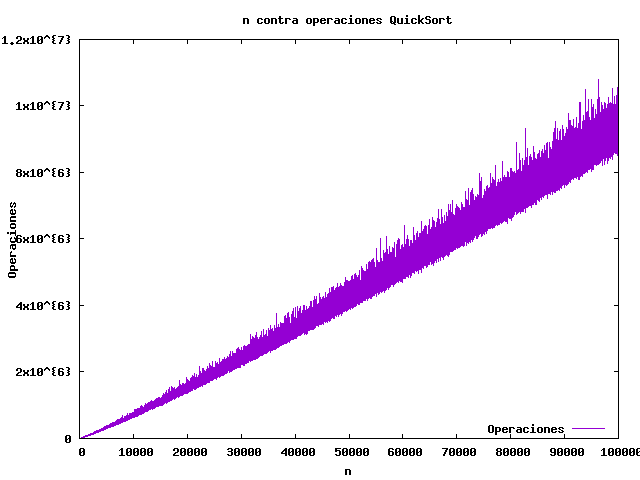
\includegraphics[width=400px,height=300px]{grafica1}
		\caption{N contra Operaciones de la solucion iterativa}
	\end{figure}
	\begin{figure}[H]
		\centering
		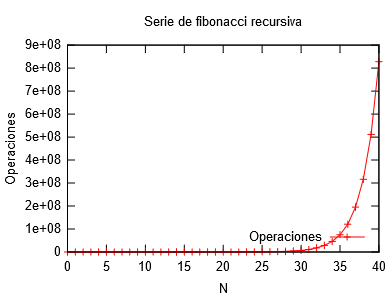
\includegraphics[width=400px,height=300px]{grafica2}
		\caption{N contra Operaciones de la solucion recursiva}
	\end{figure}
	\begin{figure}[H]
		\centering
		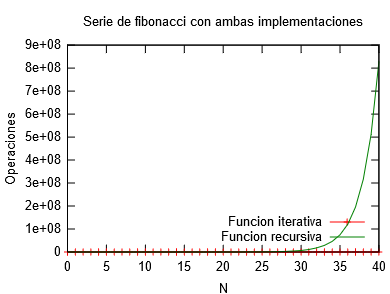
\includegraphics[width=400px,height=300px]{grafica3}
		\caption{N contra Operaciones de las dos implementaciones}
	\end{figure}
	Ahora procedemos a calcular formalmente la complejidad de la implementacion iterativa
	Empezamos calculando la complejidad temporal de cada linea:
	\begin{center}
		\begin{table}[H]
			\begin{tabular}{|l|l|l|}
				\hline
				\rowcolor[HTML]{FFCC67} 
				Codigo                           & Costo & Veces ejecutado \\ \hline
				\textit{a = 0}                    & $\O(1)$    & 1               \\ \hline
				\textit{b = 0}                    & $\O(1)$    & 1               \\ \hline
				\textit{c = 0}                    & $\O(1)$    & 1               \\ \hline						
				\textit{for(i=0;i$\leq$n;i++)} & $\O(n)$    & n+2             \\ \hline
				\textit{\  \  c = a}                 & $\O(1)$    & n               \\ \hline
				\textit{\  \  a = b}                     & $\O(1)$    & n+1               \\ \hline
				\textit{\  \  b += c}                     & $\O(1)$    & n+1               \\ \hline
				\textit{return a}                & $\O(1)$    & 1               \\ \hline
			\end{tabular}
		\end{table}										
	\end{center}			
	Lo cual nos indica que la complejidad de la solucion iterativa es lineal, es decir $T(n)\in\O(n)$. Esto lo podemos corroborar en la Figure 3 donde se puede apreciar que el numero de operaciones de la implementacion contra N crece de forma lineal.\\			
	Por otro lado, de forma experimental podemos proponer que la complejidad de la solución recursiva es: $2^N$			
	\subsection{Implementar las funciones Perfecto(N) y MostrarPerfectos(N)}
	Para el segundo conjunto de funciones, se decidio buscar los primeros 4 números perfectos, y probar todos los números hasta 10 000.
	\begin{figure}[H]
		\centering
		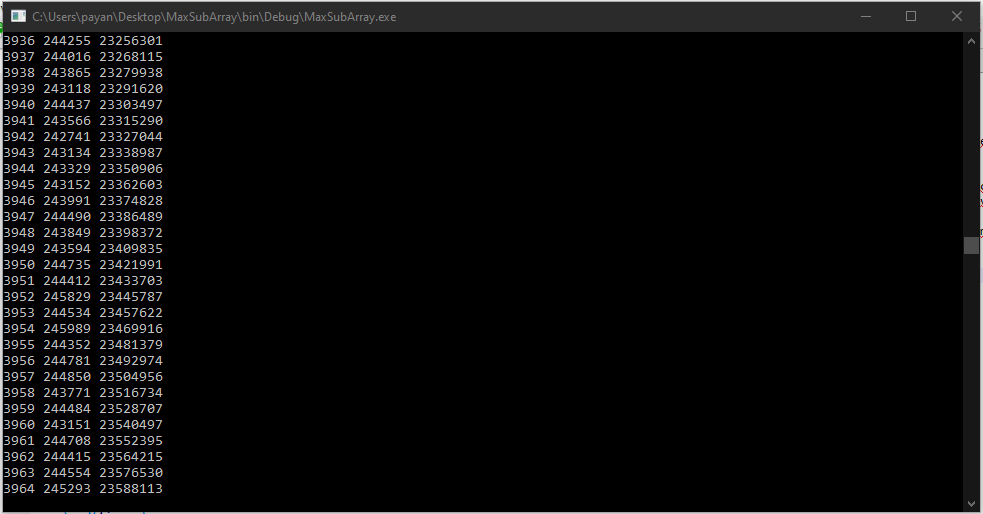
\includegraphics[width=400px,height=200px]{ejecucionSegundaParte}
		\caption{Ejecucion del programa en la seccion de prueba de números}
	\end{figure}
	\begin{figure}[H]
		\centering
		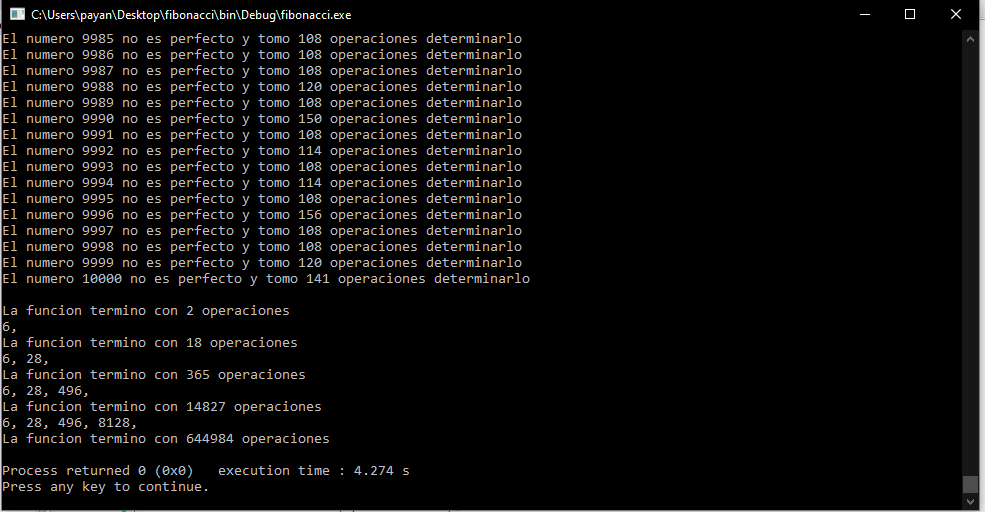
\includegraphics[width=400px,height=200px]{ejecucionTerceraParte}
		\caption{Ejecucion del programa en la seccion de obtener N perfectos}
	\end{figure}
	\begin{figure}[h!]
		\centering
		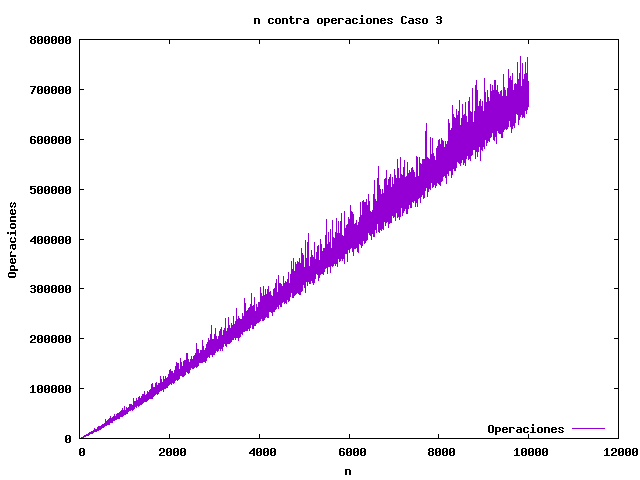
\includegraphics[width=400px,height=300px]{grafica5}
		\caption{N contra Operaciones de Perfecto(N)}
	\end{figure}
	\begin{figure}[H]
		\centering
		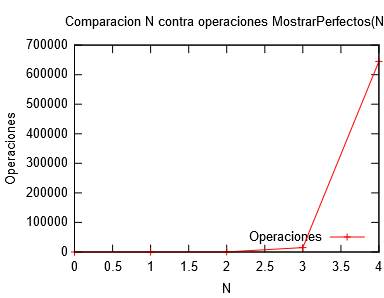
\includegraphics[width=400px,height=300px]{grafica4}
		\caption{N contra Operaciones de MostrarPerfectos(N)}
	\end{figure}
	Ahora procedemos a calcular formalmente la complejidad de la funcion Perfecto(N)
	Empezamos calculando la complejidad temporal de cada linea:
	\begin{center}
		\begin{table}[H]
			\begin{tabular}{|l|l|l|}
				\hline
				\rowcolor[HTML]{FFCC67} 
				Codigo                           & Costo & Veces ejecutado \\ \hline
				\textit{raiz = sqrt(n)}                    & $\O(1)$    & 1               \\ \hline
				\textit{suma = 1}                    & $\O(1)$    & 1               \\ \hline
				\textit{for(i=2;i$\leq$raiz;i++)} & $\O(\sqrt{n})$    & $\sqrt{n}$+2             \\ \hline
				\textit{\  \  if(n mod i == 0)}                 & $\O(1)$    & $\sqrt{n}$               \\ \hline
				\textit{\  \  \  \  if(n/i > raiz)}                     & $\O(log_2(n))$    & $log_2(n)+1$              \\ \hline
				\textit{\  \  \  \  \  \  suma += n/i}                     & $\O(1)$    & $\frac{log_2(n)}{2}$               \\ \hline
				\textit{\  \  \  \  suma+=i}                     & $\O(1)$    & $log_2(n)$               \\ \hline
				\textit{return (suma==n?1:0)}                & $\O(1)$    & 1               \\ \hline
			\end{tabular}
		\end{table}										
	\end{center}			
	Lo cual nos indica que la complejidad de la funcion Perfecto(n) es $\sqrt{n}$, es decir $T(n)\in\O(\sqrt{n})$. Esto lo podemos corroborar en la Figure 3 donde se puede apreciar que el numero de operaciones de la implementacion contra N crece acotado por abajo por $\sqrt(2)$ y acotado por arriba por $c\sqrt{n}$.\\			
	Por otro lado, de forma experimental y basado en la tabla de perfectos conocidos,podemos observar que la complejidad de la funcion MostrarPerfectos(n) crece de forma exponencial debido a que el espacio entre cada perfecto es muy grande, asimismo las formas mas optimas que ocupan el calculo de un primo p, igual tienen complejidades gigantes, debido a que es dificil hallar un primo y no todos aplican para la funcion, sin mencionar que computacionalmente cuesta muchisimo trabajo hacerlo.
	
	\section{Conclusiones}			
	\subsection{Payán Téllez René}
	Esta practica se me hizo particulamente interesante porque los algoritmos que se trataron, no fueron tan directos de implementar en un lenguaje de programación, sin mencionar que algunas graficas tuvieron muy pocos valores, debido a lo complicado que era generar mas, porque computacionalmente su complejidad es inmensa. De hecho tuve que cambiar algunas variables de int a long long int en el espacio de los contadores para que siguiera funcionando el contador sin desbordarse. Tambien vi lo interesante de un algoritmo como MostrarPerfectos que tiene una complejidad no polinomial, ya que aunque lo puedo programar tardaria horas en encontrar mas alla del perfecto 5 (de por si toma mas de 5 minutos hallar el perfecto 4) sin mencionar que le tomaria dias encontrar otros números. Tambien cuando estaba demostrando la complejidad del algoritmo recursivo de la secuencia de fibonacci, algunos nucleos del CPU de mi computadora se dispararon, lo cual fue una señal de lo complicado y tardado que se podia volver en N muy grandes.\\
	\includegraphics[height=120px,width=120px]{Rene}
	\section{Anexo}			
	\subsection{Investigar el algoritmo de Karatsuba que permite obtener la multiplicación de enteros muy grandes}
	\subsection{Resolver los siguientes problemas}
	\section{Bibliografia}
	{[}1{]}\url{http://www.lcc.uma.es/~av/Libro/CAP3.pdf}\\
	{[}2{]}\url{https://medium.com/@joseguillermo_/qu%C3%A9-es-la-complejidad-algor%C3%ADtmica-y-con-qu%C3%A9-se-come-2638e7fd9e8c}\\
		{[}3{]}\url{https://es.wikipedia.org/wiki/P_(clase_de_complejidad)}\\
		{[}4{]}\url{https://es.wikipedia.org/wiki/NP_(clase_de_complejidad)}\\
		{[}5{]}\url{https://quantdare.com/numeros-de-fibonacci/}\\
		{[}6{]}\url{https://matematicascercanas.com/2015/03/04/numeros-perfectos/}\\
		{[}7{]}\url{https://www.smartick.es/blog/matematicas/numeros/numeros-primos-criba-eratostenes/}\\		
	\end{document}